\documentclass[border=2pt]{standalone}
\usepackage{tikz}
\usetikzlibrary{arrows.meta, positioning, calc, intersections, shapes.misc}

\begin{document}
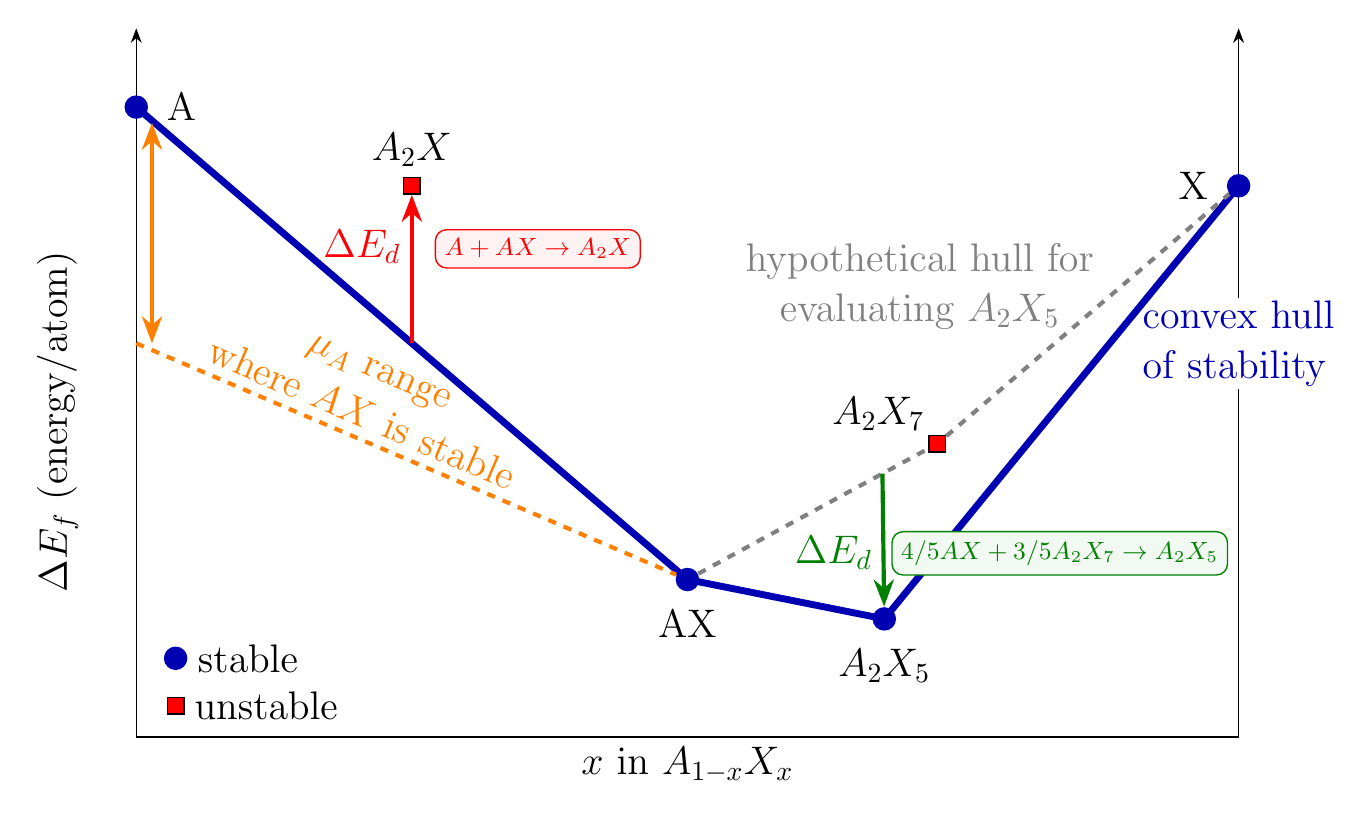
\begin{tikzpicture}[
    >=Stealth,
    point/.style={circle, fill, inner sep=3pt},
    unstable/.style={rectangle, draw, fill=red, inner sep=3pt},
    font=\Large,
    line width=0.5pt,
    reaction box/.style={rounded corners, draw=#1, fill=#1!5, text=#1, align=left, font=\small},
]
% Define the main coordinates
\coordinate (Origin) at (0,0);
\coordinate (TopLeft) at (0,8);
\coordinate (BottomRight) at (14,0);
\coordinate (TopRight) at (14,9);
\coordinate (AX) at (7,2);
\coordinate (A2X5) at (9.5,1.5);

% Axes
\draw[->] (Origin) -- ($(TopLeft)+(0,1)$);
\node[rotate=90, anchor=center] at ($(Origin)!0.5!(TopLeft)-(1,0)$) {$\Delta E_f$ (energy/atom)};
\draw (Origin) -- (BottomRight);
\draw[->] (BottomRight) -- (TopRight);
\node[below] at ($(Origin)!0.5!(BottomRight)$) {$x$ in $A_{1-x}X_x$};

% Convex hull
\node[blue!70!black, align=left, fill=white, inner sep=1pt] at (14,5) {convex hull\\of stability};
\draw[blue!70!black, line width=2.5pt, name path=hull]
    (TopLeft) -- (AX) -- (A2X5) -- (14,7);

% Stable points
\node[point, blue!70!black] (A) at (TopLeft) {};
\node[point, blue!70!black] (AX) at (AX) {};
\node[point, blue!70!black] (A2X5) at (A2X5) {};
\node[point, blue!70!black] (X) at (14,7) {};

% Labels for stable points
\node[right=3pt of A] {A};
\node[below=3pt of AX] {AX};
\node[below=3pt of A2X5] {$A_2X_5$};
\node[left=3pt of X] {X};

% Unstable points
\node[unstable] (A2X) at ($(A)!0.5!(AX)+(0,2)$) {};
\node[unstable] (A2X7) at ($(A2X5)!0.15!(X)+(0,1.4)$) {};

% Labels for unstable points
\node[above=0pt of A2X] {$A_2X$};
\node[above left=-3pt of A2X7] {$A_2X_7$};

% Delta E arrows
\coordinate (A2X_hull) at ($(A)!0.5!(AX)$);
\draw[->, red, line width=1.5pt] (A2X_hull) -- (A2X) node[pos=0.65, left, red] {$\Delta E_d$};
\node[reaction box=red] at ($(A)!0.5!(AX)+(1.6,1.2)$) {$A + AX \to A_2X$};

% Hypothetical hull
\draw[gray, dashed, line width=1.5pt] (AX) -- (A2X7) -- (X);
\node[gray, above=3cm of $(A2X5)!0.1!(X)$, align=center] {hypothetical hull for\\evaluating $A_2X_5$};

% Delta E_d arrow for hypothetical hull
\coordinate (hull_midpoint) at ($(AX)!0.78!(A2X7)$);
\draw[->, green!50!black, line width=1.5pt] (hull_midpoint) -- (A2X5) node[pos=0.6, left, green!50!black] {$\Delta E_d$} node[reaction box=green!50!black,pos=0.6, right=0.1, line width=0.5pt] {$4/5 AX + 3/5 A_2X_7 \to A_2X_5$};

% Chemical potential range (orange line)
\coordinate (OrangeLow) at (0,5);
\draw[orange, dashed, line width=1.5pt] (OrangeLow) -- (AX)
    node[pos=0.4, above, sloped, align=center] {$\mu_A$ range\\where $AX$ is stable};

% Orange double arrow
\draw[<->, orange, line width=1.5pt] ($(TopLeft)+(0.2,-0.2)$) -- ($(OrangeLow)+(0.2,0)$);

% Legend
\node[point, blue!70!black, label={right:stable}] at (0.5,1) {};
\node[unstable, label={right:unstable}] at (0.5,0.4) {};

\end{tikzpicture}
\end{document}
